\section{Na\"ive implementation}
The na\"ive implementation was implemented first. This was done using only standard Python operations, however, numpy arrays were used as well as the numpy.zeros and numpy.empty for creating the arrays. 

In the na\"ive version of the code a function is needed which creates histogram information based on an image and parameters given as arguments. This was used by both the noise remover function and the equalise histogram function. \\

The noise remover function was implemented as follows. First it creates a histogram of the input image. Based on the histogram it identifies a threshold value. This is done by first identifying the highest and lowest bin-value which has a frequency of more than a specified "recognition value", which was set to 10 in this mini project. Afterwards it calculates the threshold by setting it equal to the lowest value identified plus a fraction of the interval between the lowest and highest value identified. The faction is determined by an argument, which is set equal to $ 0.1 $ in this mini project. After the threshold has been identified it is applied to the pixels in the image. A part of the algorithm identifies the pixels with values lower than the threshold and saves the pixel coordinates of the pixels. The saved pixels are then reconstructed from neighbouring pixels which have already been reconstructed or pixel that was not thresholded, in an iterative fashion. Once all thresholded pixels have been reconstructed the reconstructed image is returned. \\

The equalise histogram function initially has the same algorithm for finding the lowest and highest bin values in the histogram of the input image as the noise remover function has. Once those values are obtained the histogram is stretched such that the lowest value is moved to $ 0 $ and the highest to $ 255 $ which is the max value of the pixel values. This is done as shown in \autoref{eq:hist_stretch}.

\begin{equation}\label{eq:hist_stretch}
	\text{New~pixelValue} (\text{pixelValue-lowVal})\cdot\frac{255}{\text{higVal-lowVal}}
\end{equation}


As a final step all pixel values above $ 255 $ or below $ 0 $ are set to $ 255 $ or $ 0 $ respectively.

\begin{figure}[h]
\centering
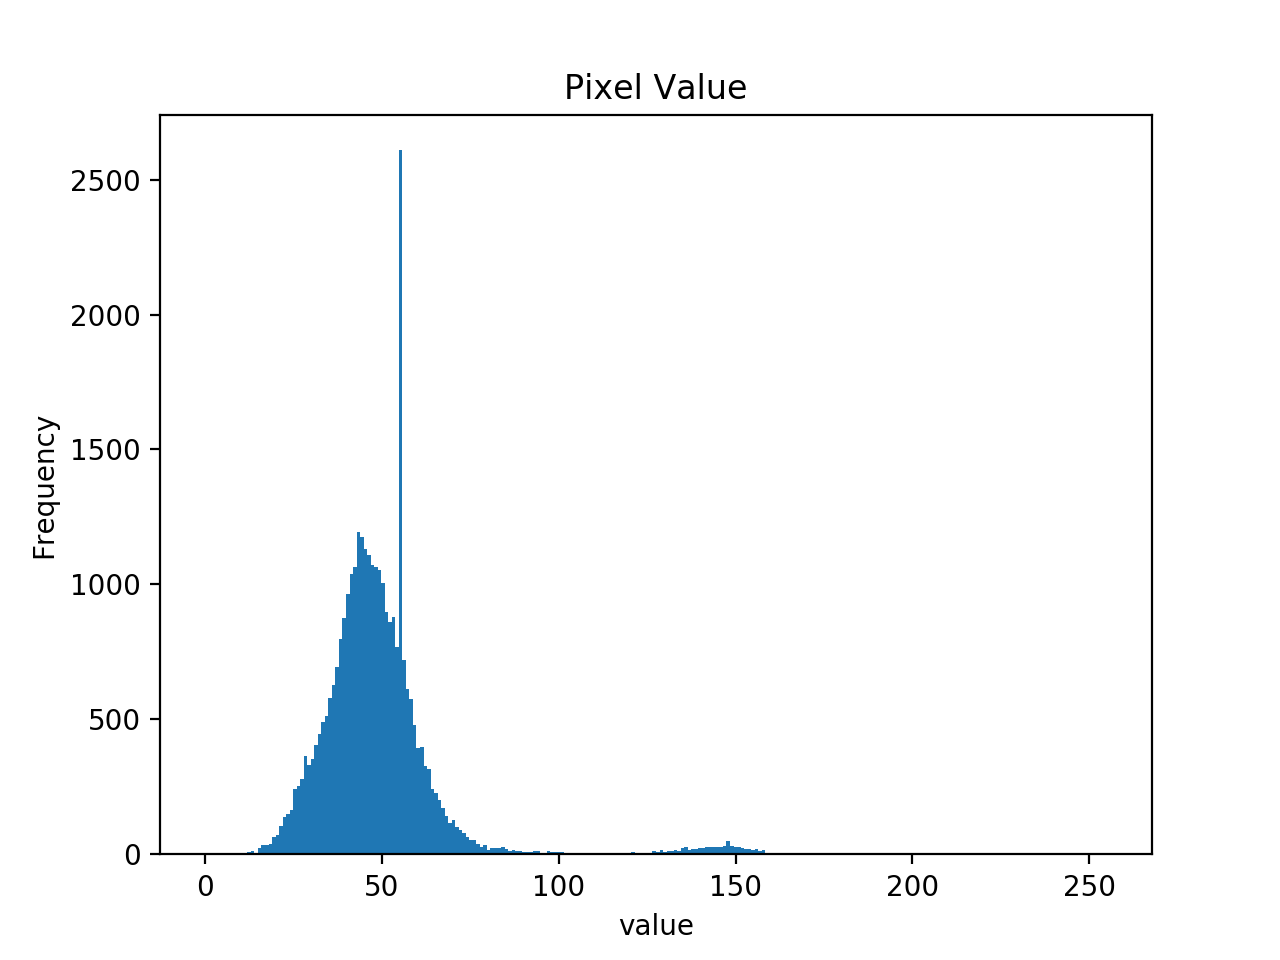
\includegraphics[width=0.7\textwidth]{figures/hist_before.png}
\caption{The histogram before applying the functions.}
\label{fig:histBif}
\end{figure}

\noindent
After implementing the code it is run on a single image to verify that it works. During this process the matplotlib.pyplot module was used to plot histograms. During the first run it became clear that something in the code was not working as intended. \autoref{fig:histBif} shows the histogram of the image before any of the functions were applied. According to the method used for reconstruction, it can be expected that there will be a clear cut in the histogram and that all the values lower will be zero. It is also expectable that a peak will occur near right at the cut-off value because the pixels which need reconstruction are reconstructed from neighbours which are likely to have close to the same pixel values. However, the plotted histogram after reconstruction was as shown in \autoref{fig:histSpill}.

\begin{figure}[h]
\centering
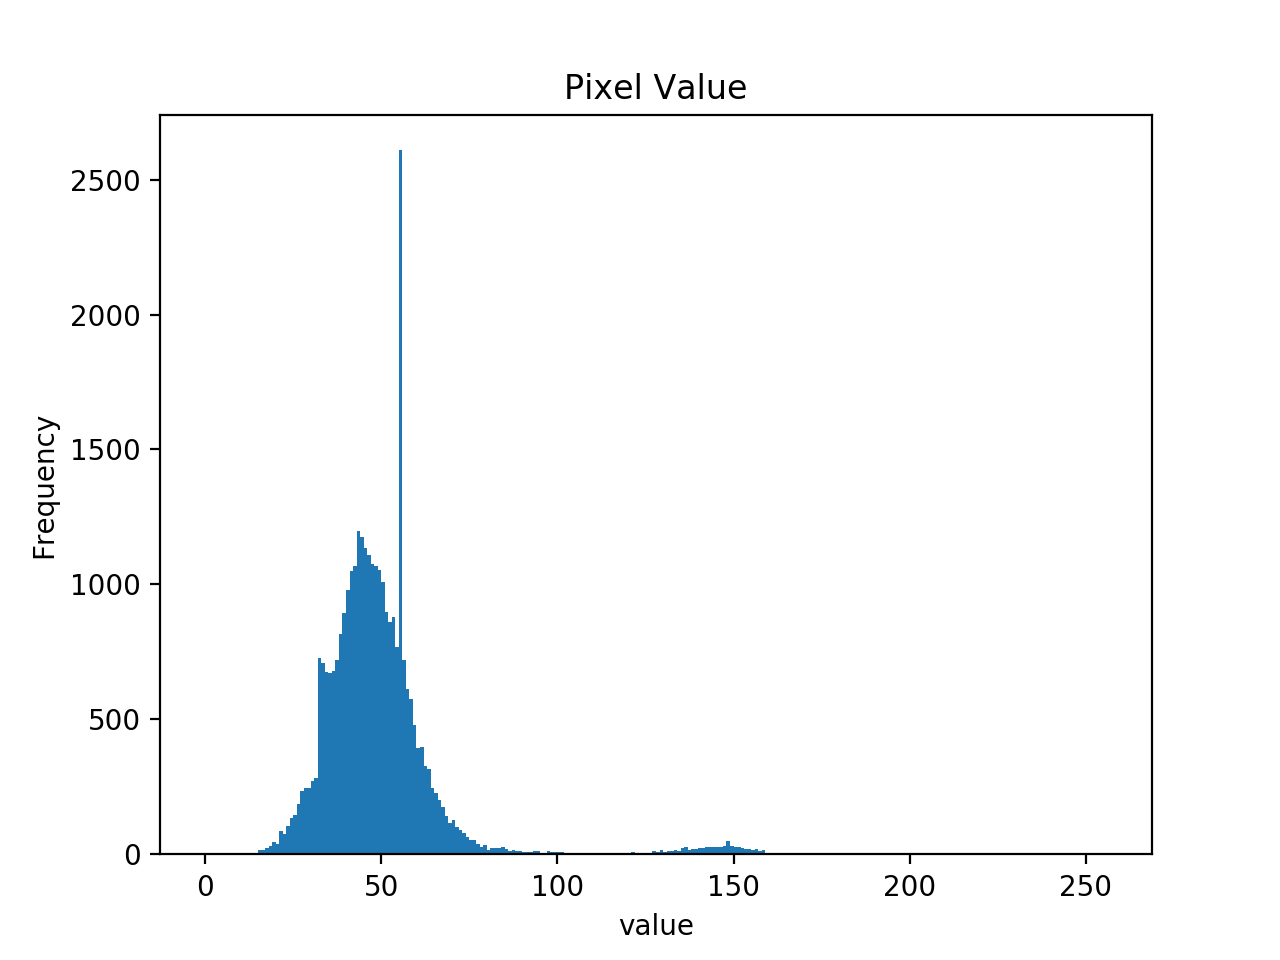
\includegraphics[width=0.7\textwidth]{figures/hist_spill.png}
\caption{The histogram of the image after applying the noise remover function, which reconstructs pixels.}
\label{fig:histSpill}
\end{figure}

\noindent
As it can be seen by comparing the two histograms in \autoref{fig:histBif} and \autoref{fig:histSpill} the peak does indeed occur, however, the pixels "spill" across the threshold value. By closer examination of the code it was discovered that this was caused due to a programming mistake. The mistake was that the values used for reconstruction were obtained from the original image and not from the reconstructed image. Once this mistake was corrected the histogram was as expected as shown in \autoref{fig:histFine}. 

\begin{figure}[h]
\centering
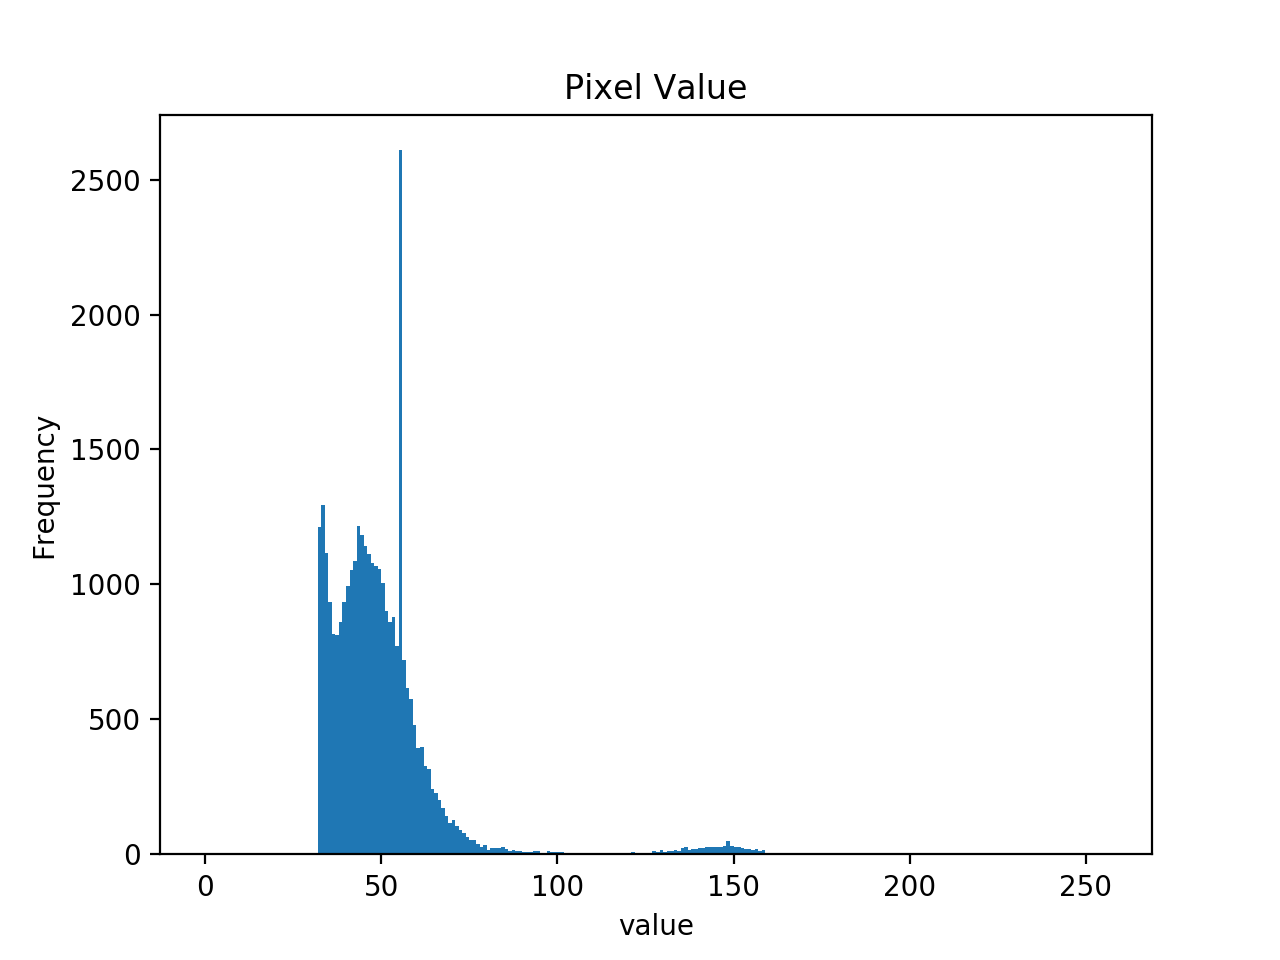
\includegraphics[width=0.7\textwidth]{figures/hist_nicespacing.png}
\caption{The histogram of the image after applying the noise corrected remover function.}
\label{fig:histFine}
\end{figure}

\noindent
After obtaining the reconstructed image histogram stretching was done by applying equalise histogram function. The histogram of the resulting image can be seen in \autoref{fig:histEq}. The figure shows that the histogram stretching is conducted successfully. 

\begin{figure}[h]
\centering
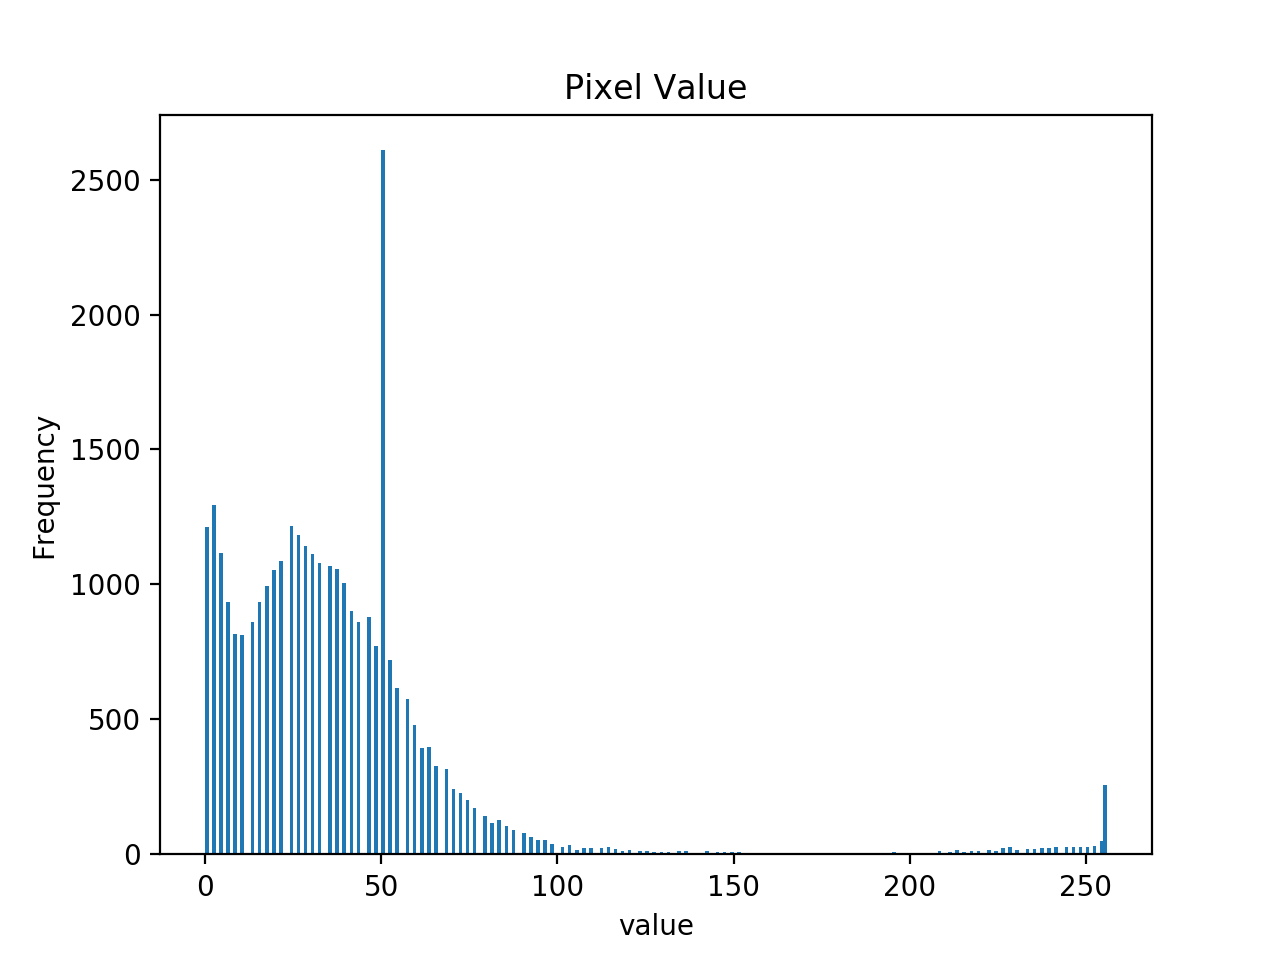
\includegraphics[width=0.7\textwidth]{figures/hist_equal.png}
\caption{The histogram of the image after applying the equalise histogram function.}
\label{fig:histEq}
\end{figure}

\noindent
The final code of the na\"ive implementation is shown in \autoref{AppNaive}.